% Repository:  https://github.com/chiehrosswang/TRB_LaTeX_tex
%
% Transportation Research Board conference paper template
% version 4.0 Lite (updates made to be compatible in Overleaf and ShareLaTeX)
%
%
% When numbered option is activated, lines are numbered.
\documentclass[numbered]{trbarticle}
\usepackage{graphicx}
\usepackage{booktabs}

\newread\somefile
\usepackage{xparse}

\usepackage{natbib}
\bibliographystyle{unsrtnat}
\setcitestyle{round}

% \usepackage[colorlinks=true,linkcolor=blue,citecolor=blue]{hyperref}
% For TRB version hide links
\usepackage[hidelinks]{hyperref}

% Put here what will go to headers as author
\AuthorHeaders{}
\title{Calibrating Ramp Meter Queue Length Models: Evidence from Utah}

% TODO: add macros for easier formatting of \author.
\author{%
    \textbf{Tanner Daines}\\
  \textit{}
  \\
  BYU\\
  \href{mailto:tdaines@byu.edu}{\nolinkurl{tdaines@byu.edu}}\\
  \hfill\break
    \textbf{Gregory Macfarlane}\\
  \textit{}
  \\
  BYU\\
  \href{mailto:gregmacfarlane@byu.edu}{\nolinkurl{gregmacfarlane@byu.edu}}\\
  \hfill\break
    \textbf{Grant Schultz}\\
  \textit{}
  \\
  BYU\\
  \href{mailto:gschultz@byu.edu}{\nolinkurl{gschultz@byu.edu}}\\
  \hfill\break
  }

% If necessary modify the number of words per table or figure default is set to
% 250 words per table
% \WordsPerTable{250}

% If words are counted manually, put that number here. This does not include
% figures and tables. This can also be used to avoid problems with texcount
% program i.e. if one does not have it installed.
\TotalWords{}

\begin{document}
\maketitle


\section{Abstract}
This is where the abstract should go.
\hfill\break%
\hfill\break%
\noindent\textit{Keywords}: 
\newpage

\hypertarget{intro}{%
\section{Introduction}\label{intro}}

As traffic on freeways continues to rise, developing a reliable method to regulate the flow of vehicles onto the freeway has become increasingly important. A primary method that was first implemented in the 1960s is the ramp meter. A ramp meter is a traffic signal that is placed on the freeway on-ramp, designed to control the rate at which vehicles enter the freeway and therefore prevent it from exceeding capacity. Although ramp meters may improve freeway traffic conditions, they often generate a queue, causing vehicles to wait on the ramp prior to entering the freeway.

Research has previously been done to estimate the queue length at freeway on-ramps, but most conclude that while certain methods improve queue size estimation, each possess shortcomings that would prevent it from being widely implemented across many ramps without significant calibration and cannot easily be used in real-time. This paper aims to improve these previously developed methods, thus providing algorithms that more accurately report the expected queue length on any given on-ramp that utilizes ramp metering.

This paper will focus on estimating the queue length of two on-ramps in Davis and Salt Lake counties in Utah. The ramps chosen for analysis are the northbound on-ramp to I-15 at Layton Parkway in Davis County and the southbound on-ramp at Bangerter Highway in Salt Lake County.

Two methods to estimate queue length are discussed in this paper, including a conservation model and a Kalman filter model. The Kalman filter model includes several variations to find a method that most accurately reflects field-observed queue lengths. This paper will discuss methods by which both the conservation and Kalman filter models can be used to estimate queue length real-time on freeway on-ramps. Various components of the ramp such as the number of lanes, the ramp length, its traffic volume and occupancy, and the metering rate will be considered. Throughout this paper, a literature review will explain the methods previously utilized to measure ramp meter performance and queue length and the methodology used to collect and analyze the data. Following this, a discussion of the results will be presented, after which the paper will conclude with a summary of all items discussed.

\hypertarget{literature-review}{%
\section{Literature Review}\label{literature-review}}

When freeway operations consistently deteriorate during peak hours, ramp meters are often implemented on the on-ramp, thus regulating the flow of vehicles entering the freeway. By controlling the flow of vehicles onto the freeway, motorists can travel in more favorable traffic conditions, which can reduce crashes, improve overall travel time, and lower emissions \citep{papageorgiou2002freeway}. Although conditions on the freeway may improve when ramp meters are implemented, this often leads to increased wait time on the on-ramp. Several ramp metering algorithms have been used in an attempt to find a balance between freeway and ramp operations, though much remains to be accomplished (Liu et al.~2012). For example, Minnesota implemented ramp meters in 1969, and in the fall of 2000---at the request of citizens in the Minneapolis-St.~Paul area---the meters were shut off for 8 weeks to analyze whether freeway conditions were superior with the ramp meters (Levinson and Zhang 2004). To the surprise of some traffic analysts, some areas of the Twin Cities showed decreased travel time without the ramp meters, though the results mostly showed that travel delay, average speed, and travel time performed significantly better with the ramp meters in use. Other areas throughout both the United States have shown similar results. The Seattle Bottleneck algorithm, used in many locations, has also reduced crash rates and average travel time (Jacboson et al.~2006). Thus, in order to best understand the benefits of ramp meters, it is imperative that their function be established.

There are two primary classifications of ramp meters: pre-timed meters and traffic-responsive meters (Jacobson et al.~2006). Pre-timed meters operate at a set rate based on historical data. This type of metering has proven effective when traffic volumes are easily predictable. However, when sudden changes in traffic operations occur, pre-timed meters often fail to account for the change without manual intervention. Traffic-responsive metering on the other hand relies on real-time data collection through the use of loop detectors, which can be placed within the pavement or in the form of traffic cameras. Due to the extensive amount of data being collected, the initial calibration of traffic-responsive meters can prove to be time consuming; however, once effectively implemented, they can mitigate congestion based on the data received on the ramp (Jacobson et al.~2006).

By using loop detectors on the ramps, time occupancy and traffic volume data are gathered. Occupancy refers to the percent of time a point on the road is occupied by a vehicle; for example, if no vehicle passes over the detector during a given time period, the occupancy would be 0 percent, whereas if a vehicle was detected passing over the detector during half of that same time period, the time occupancy would show 50 percent (\citet{wu2009experiment}). Several studies have been conducted to use the data gathered by loop detectors to estimate the queue length on metered on-ramps. Vigos et al.(2006), Liu et al.~(2007), and \citet{wu2009experiment} (2009) utilize the loop detector data to estimate queue length with two proposed methods, including a conservation model and a Kalman filter model. The conservation model assumes that the number of vehicles entering and exiting the ramp throughout a given time period is the same. The Kalman filter model is based on the conservation model, but uses additional ramp characteristics and a Kalman filter coefficient ``K'' to improve the queue length estimate provided by the conservation model. Wu et al.~(2009) also use the Highway Capacity Manual (HCM) back of queue method, however it proved to be ineffective, and will not be discussed in detail in this literature review. The original equations developed for the conservation model and Kalman filter algorithms required the volume entering and exiting the ramp to be equal, but through analysis of the data, Wu et al.~(2009) found that the volumes were not balanced over time.

\hypertarget{using-a-volume-balancing-ratio}{%
\subsection{Using a Volume-Balancing Ratio}\label{using-a-volume-balancing-ratio}}

Many difficulties are introduced when relying solely on ramp detector data. One difficulty in particular is that vehicles can be double-counted or missed altogether depending on the location of the vehicle passing over the detector (Wu et al.~2008). Because of this potential for error, the original conservation model equation and Kalman filter equation were modified by Wu et al.~2008 to balance the volumes entering and exiting the ramp, which is shown by a volume-balancing ratio ``C'' in each equation. Equation 1 is the conservation model equation with the volume-balancing ratio included, and Equation 2 and Equation 3 are the equations used for the Kalman filter method with the volume-balancing ratio.

The Kalman filter model applied by \citet{wu2009experiment} is as follows:

\begin{equation}
q_i = q_{i-1} + c_i + k (\hat{q}_i - q_{i-1})
  \label{eq:kalman}
\end{equation}

Using the volume-balancing ratio previously mentioned, it is presumed that the conservation model and Kalman filter algorithms will produce more accurate queue length estimates, which can then be used to calculate the expected vehicle wait time. \citet{wu2009experiment} explain that the volume-balancing ratio may be set as a constant value or may be calculated in real time. Prior to incorporating this volume-balancing ratio, when \citet{wu2009experiment} utilized Equation 2 to find the queue length estimate based on the occupancy data, they found the correlation between the estimated queue length and the time occupancy to be only 0.63. This research also concluded that the relationship between volume data from the detector and the estimated number of vehicles is nonlinear, as the results gave a correlation coefficient of merely 0.18 between the two variables. Therefore, it is likely there are other factors outside the capability of this equation that affect the queue length such as detector error, driver distraction, poor weather, and traffic incidents.

However, in analyzing 20 data sets from ramp meters in Milwaukee, Wisconsin, \citet{wu2009experiment} found that the volume-balancing ratio improved both the Kalman filter and the conservation models considerably in nearly all cases, and in only a select few cases were slightly more errors introduced. These errors were found to occur in the Kalman filter models because when the volume-balancing ratio is close to 1 (the detector volume entering and exiting the ramp are nearly equal), the Kalman filter coefficient K is also close to zero, but the equation still adds queue length to the estimate from the coefficient K, which would introduce additional error. In contrast, when the volume-balancing ratio is not close to 1, the Kalman filter equation yield more reliable results than the conservation model. Overall, \citet{wu2009experiment} found that both the Kalman filter and conservation model, especially when using the volume-balancing ratio, provide generally accurate estimates of the actual queue length.

\hypertarget{determination-of-k}{%
\subsection{Determination of K}\label{determination-of-k}}

Research previously conducted on estimating the queue length on on-ramps using a Kalman filtering method has yielded varied and generally inconclusive results with respect to which value of K should be used at any given on-ramp, especially for real-time estimation. Vigos et al.~(2006) was of the first to use the Kalman filtering equation to estimate the queue length at metered on-ramps. The estimation for this research was done using microscopic simulation, and it concluded that while K ranged from {[}0.1, 0.25{]} in their analysis, the optimum value to be used for K is ``0.22 for one detector and 0.5 for all other detector numbers'' Vigos et al.~(2006). However, no field testing was performed in this analysis. Liu et al.~(2007) appears to have used a linear regression model to calculate K by using the passage and queue occupancy, and they concluded that the Kalman filter yielded the most accurate results for ramps that were determined to have significant error (larger than 2 percent) between the volume detected by queue and passage detectors. Finally, Wu et al.~(2009) proposed calculating K by minimizing the root-mean sqaured error (RMSE) between the field-collected queue length and the estimated queue length with the Kalman filter for each peak period at each ramp. Wu et al.~(2009) again confirm that the Kalman filter outperforms the conservation model when there is significant error between the queue and passage detectors, because the Kalman filter model can correct itself. Wu et al.~(2009) confirm that the Kalman filter coefficient would require significant calibration for each ramp metering location and for each peak period. Thus, manually collected data would be required for each additional ramp that is desired to be studied, which limits the feasibility of using the Kalman filter in real-time.

\hypertarget{relationship-between-k-and-traffic-analysis-parameters}{%
\subsection{Relationship between K and Traffic Analysis Parameters}\label{relationship-between-k-and-traffic-analysis-parameters}}

This paper will seek to expound on previously performed research by finding ways the Kalman filter coefficient K can be correlated with various traffic analysis parameters that can be calculated directly from the detector data. If a reliable correlation between these parameters and K can be found, the queue length can then calculated in real time with the Kalman filter equation.

Each metered on-ramp in Utah has three detector locations in each lane. These detectors include at the excessive queue (EQ), which is located shortly after the entrance to each ramp, the intermediate queue (IQ), located roughly in the middle of the on-ramp, and the passage queue (PQ), located directly after the ramp meter signal. Both volume and occupancy data are collected by these detectors in 60-second increments at each of these locations. The variable ramp metering rate is also updated every 60 seconds. The length of the ramp and number of lanes on the ramp are also known by observation. Using these data, additional traffic analysis parameters such as the traffic density (in units of veh/mi/ln) and flow (in units of veh/hr) can be calculated.

\hypertarget{methodology}{%
\section{Methodology}\label{methodology}}

This section will describe the methodology used in collecting and analyzing the data used in this paper. The ramps used for analysis and the metering period will be explained, and the data collected in the field and by the detectors will also be discussed.

\hypertarget{data-collection}{%
\subsection{Data Collection}\label{data-collection}}

Two on-ramps to I-15 in Davis and Salt Lake counties in Utah were chosen for data collection and analysis. These ramps include the northbound on-ramp at Layton Parkway in Davis County and the southbound on-ramp at Bangerter Highway in Salt Lake County. Data were collected during several periods, including August and September 2020, and April 2021. At Layton Parkway, 19 days of data were collected, while 5 days of data were collected at Bangerter Highway. These ramps were metered only during the PM peak period, with metering taking place between 4:00 - 6:30 PM at Layton Parkway and 3:30 - 5:45 PM at Bangerter Highway.

As mentioned, the loop detectors at the EQ, IQ, and PQ locations collect both volume and occupancy data and are recorded in 60-second increments. In addition, the variable ramp meter rate (in units of veh/hr) for each minute is included with the detector data. The detector data used in this paper were obtained through UDOT for each data collection period.

The data collected manually was also completed in 60-second increments during the metered period and includes the number of vehicles in each lane at the EQ detector, the queue length at the ramp meter signal, and the total number of other vehicles on the ramp that have not yet reached the queue. The ramp length and the number of lanes at the ramp meter signal were also recorded.

\hypertarget{data-analysis}{%
\subsection{Data Analysis}\label{data-analysis}}

While beginning to analyze the data, it was discovered that the time stamps for the field and detector data were misaligned for each ramp. This significantly reduced the accuracy of the queue length estimates, but this was resolved by shifting the field data either backwards or forwards up to three minutes to best match the detector data based on the minimum RMSE found for the number of vehicles entering the ramp.

In order to better analyze the data, rather than finding an optimum K for an entire peak period at each ramp as was done in Wu et al.~(2009), the data were grouped into 15-minute bins during each day. Doing so allows for more specific optimization of K and provides additional observations that can be used to compare each K with the traffic analysis parameters. The K for each period is found by minimizing the RMSE between the queue length from the field data and that estimated by the Kalman filter equation. The optimized K, average EQ, IQ, and PQ occupancy, metering rate, density, and flow were then computed for each 15-minute period. The data were then analyzed by finding different ways in which the optimized K values were correlated to different traffic analysis parameters.

\hypertarget{applications}{%
\section{Applications}\label{applications}}

Some \emph{significant} applications are demonstrated in this chapter.

\begin{verbatim}
## Warning in file_diff_dbl(chr): NAs introduced by coercion
\end{verbatim}

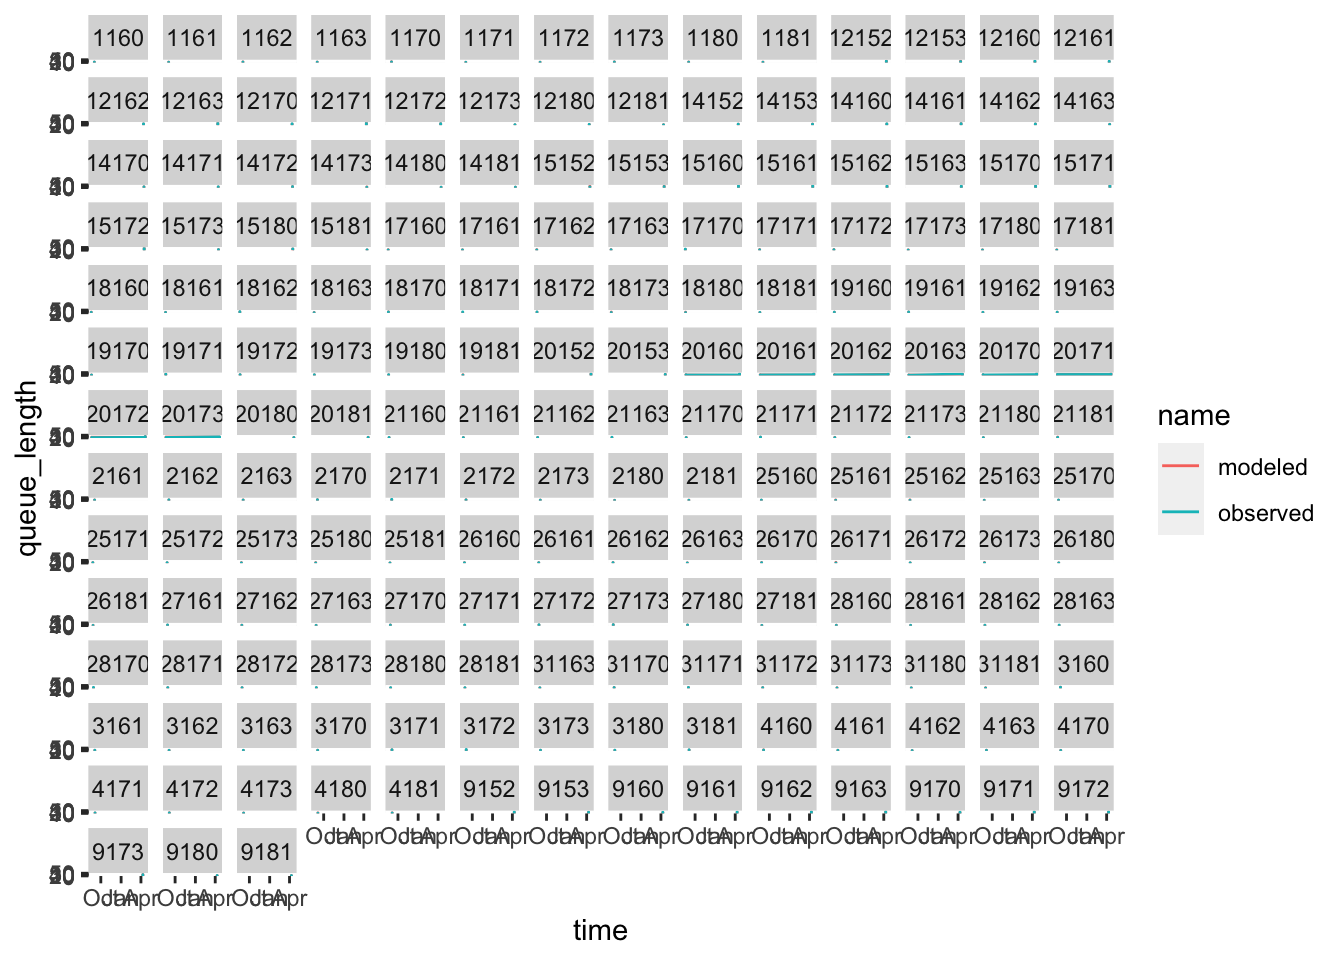
\includegraphics{ramp_meters_files/figure-latex/unnamed-chunk-1-1.pdf}

\hypertarget{section}{%
\subsection{}\label{section}}

\hypertarget{results}{%
\section{Results}\label{results}}

Linear regression models were created based on the traffic analysis parameters of occupancy, flow, and density, as seen in Table \ref{tab:models-summ}. This table compares..

\begin{verbatim}
## Warning in file_diff_dbl(chr): NAs introduced by coercion
\end{verbatim}

A cluster analysis was also performed, which compares the flow versus the density for each 15-minute period and then compares the average K for each cluster, as seen in Table \ref{tab:cluster-analysis-tab} and Figure \ref{fig:cluster-analysis-fig}. It was found that in general, the higher the traffic density, the more accurate the conservation model became, in other words, K began to approach 0. As traffic density decreased on the ramp, K began to increase closer to 1. With this information, a heuristic model can be developed to predict the queue length of vehicles at the metered on-ramp based on the traffic density on the ramp.

\begin{verbatim}
## Warning in file_diff_dbl(chr): NAs introduced by coercion
\end{verbatim}

\begin{verbatim}
## Warning in file_diff_dbl(chr): NAs introduced by coercion
\end{verbatim}

\begin{verbatim}
## Warning in file_diff_dbl(chr): NAs introduced by coercion
\end{verbatim}

\includegraphics{ramp_meters_files/figure-latex/pdata_plot-1.pdf}

\hypertarget{linear-regression}{%
\subsection{Linear Regression}\label{linear-regression}}

\hypertarget{cluster-analysis-heuristics}{%
\subsection{Cluster Analysis / Heuristics}\label{cluster-analysis-heuristics}}

\hypertarget{final-words}{%
\section{Final Words}\label{final-words}}

We have finished a nice book.

\hypertarget{final-words-1}{%
\section{Final Words}\label{final-words-1}}

We have finished a nice book.

\hypertarget{acknowledgements}{%
\section*{Acknowledgements}\label{acknowledgements}}
\addcontentsline{toc}{section}{Acknowledgements}

This research was funded by the Utah Department of Transportation. The authors
alone are responsible for the preparation and accuracy of the information, data,
analysis, discussions, recommendations, and conclusions presented herein. The
contents do not necessarily reflect the views, opinions, endorsements, or
policies of the Utah Department of Transportation or the US Department of
Transportation. The Utah Department of Transportation makes no representation or
warranty of any kind, and assumes no liability therefore.

Cory Ward and James Umphress provided indispensable data preparation work.

\newpage
\bibliography{book.bib}


\end{document}
